\section{Linear Estimation}
% ========================================================================================
\begin{emphbox}
	$t$ is now the unknown parameter $θ$, we want to estimate $y$ and $\vec x$ is the input vector...  review regression problem $\vec y = \ma A \vec x$ (we solve for $\vec x$), here we solve for $\vec t$, because $\vec x$ is known (measured)! Confusing...\\
	1. Training $\ra$ 2. Estimation\\
	Training: We observe $y$ and $\vec x$ (knowing both) and then based on that we try to estimate $y$ given $\vec x$ (only observe $\vec x$) with a linear model $\hat y=\vec x^\top\vec t$
\end{emphbox}

\begin{sectionbox}
	\begin{emphbox}
		Estimation: $\hat y = \vec x^\top \vec t + m$ \quad or \quad $\hat y = \vec x^\top \vec t$\\
	\end{emphbox}
	Given: $N$ observations $(y_i, \vec x_i)$, unknown parameters $\vec t$, noise $m$\\
	$\vec y = \mat{y_1 \\ \svdots \\ y_n}$ \quad $\ma X = \mat{\vec{x}_1^\top \\ \svdots \\ \vec{x}_n^\top}$ \qquad Note: $\hat y ≠ y$!!\\
	Problem: Estimate $y$ based on given (known) observations $\vec x$ and unknown parameter $\vec t$ with assumed linear Model: $\hat y = \vec x^\top \vec t$\\
	Note $y = \vec x^\top \vec t + m \ra y = \vec x^{'\top} \vec t'$ with $\vec x'=\vect{\vec x \\ 1}$,\quad$t'=\vect{\vec t \\ m}$\\
	\\
	Sometimes in Exams: $\hat y = \vec x^\top \vec t \Leftrightarrow \hat{\vec x} = \ma T^\top \vec y$\\ estimate $\vec x$ given $\vec y$ and unknown $\ma T$\\
\end{sectionbox}

\begin{sectionbox}
	\subsection{Least Square Estimation (LSE)}
	Tries to minimize the square error for linear Model: $\hat y_{\ir LS} = \vec x^\top \vec t_{\ir LS}$\\
	Least Square Error: $\min \left[ \sum\limits_{i=1}^N (y_i - \vec x_i^\top \vec t)^2 \right] = \min\limits_{\vec t} \norm{\vec y - \ma X \vec t}$\\
	\begin{emphbox}
		$\vec t_{\ir LS} = (\ma X^\top \ma X)^{-1} \ma X^\top \vec y$\\
	\end{emphbox}
	$\hat{\vec y}_{\ir LS} = \ma X \vec t_{\ir LS} \in span(X)$

	\textbf{Orthogonality Principle:} $N$ observations $\vec x_i ∈ \R^d$ \\ $\ma Y − \ma X\ma T_{\ir LS} ⊥ \operatorname{span}[\ma X] \Leftrightarrow \ma Y - \ma X \ma T_{\ir LS} ∈ \operatorname{null}[\ma \X^\top]$, thus\\
	$\ma X^\top (\ma Y − \ma X \ma T_{\ir LS} ) = 0$ and if $N > d ∧ \operatorname{rang}[\ma X] = d$:\\ $\ma T_{\ir LS} = (\ma X^\top \ma X)^{-1} \ma X^\top \ma Y$
\end{sectionbox}



\begin{sectionbox}
	\subsection{Linear Minimum Mean Square Estimator (LMMSE)}
	Estimate $y$ with linear estimator $\vec t$, such that $\hat y = \vec t^\top \vec x + m$ \\
	Note: the Model does not need to be linear! The estimator is linear!
	\begin{emphbox}
		$\hat y_{\ir LMMSE} = \underset{t,m}{\arg \min} \E\left[ \norm{\vec y - ( \vec t^\top \vec x+ m)}_2^2 \right]$
	\end{emphbox}
	If Random joint variable $\vec z = \vect{\vec x \\ y}$ with \\ $\vec {μ}_{\vec z} = \vect{\vec{μ}_{\vec x} \\ μ_y}$ and $\ma C_{\vec z} = \mat{\ma C_{\vec x} & \vec c_{\vec xy} \\ c_{y\vec x} & c_y}$ then\\
	LMMSE Estimation of $y$ given $x$ is\\
	$\hat y = μ_y+\vec c_{y\vec x} \ma C_{\vec x}^{-1}(\vec x-\vec{μ}_{\vec x}) = \underbrace{\vec c_{y\vec x} \ma C_{\vec x}^{-1}}_{=\vec t^\top}\vec x - \underbrace{μ_y + \vec c_{y\vec x} \ma C_{\vec x}^{-1}\vec{μ}_{\vec x}}_{= m}$\\
	Minimum MSE: $\E\left[ \norm{\vec y - (\vec x^\top \vec t + m)}_2^2 \right] = c_y - c_{y\vec x} C_{\vec x}^{-1}\vec c_{\vec xy}$\\
	\\
	\textbf{Hint:} First calculate $\hat y$ in general and then set variables according to system equation.\\
	\textbf{Multivariate:} $\hat{\vec y} = \ma T_{\ir LMMSE}^\top \vec x$ \qquad $ \ma T_{\ir LMMSE}^\top = \ma C_{\vy \vx} \ma C_{\vx}^{-1}$\\
	\rule{\columnwidth}{0.5pt}
	\\
	If $\vec \mu_{\vec z} = \vec 0$ then\\
	Estimator $\hat y = \vec c_{y, \vec x} \ma C^{-1}_{\vec x} \vec x$\\
	Minimum MSE: $\E[c_{y,\vec x}] = c_y - \vec t^\top \vec c_{\vec x,y}$
\end{sectionbox}



\begin{sectionbox}
	\subsection{Matched Filter Estimator (MF)}
	For channel $\vec y = \vec hx + \vec v$, Filtered: $\vec t^\top \vec y = \vec t^\top\vec h x + \vec t^\top \vec v$\\
	Find Filter $\vec t^\top$ that maximizes SNR $= \frac{\norm{ \vec h x}} {\norm{\vec v}}$\\
	$\ma t_{\ir MF} = \underset{t}{\max} \left\{ \frac{\E\left[ (\vec t^\top \vec h x)^2 \right] }{\E\left[ (\vec t^\top \vec v)^2 \right] } \right\}$\\
	\\
	In the lecture (estimate $\vec h$):\\
	$\ma T_{\ir MF} = \underset{T}{\max} \left\{ \frac{\left| \E\left[ \hat{\vec h}^H \vec h \right] \right|^2}{\operatorname{tr}\left[ \Var[\ma T \vec n]\right] } \right\}$\\
	$\hat{\vec h}_{\ir MF} = \ma T_{\ir MF} \vec y$ \qquad $\ma T_{\ir MF} \propto \ma C_{\vec h} \ma S^H \ma C^{-1}_{\vec n}$

\end{sectionbox}





\begin{sectionbox}
	\subsection{Example}

	\begin{center}
		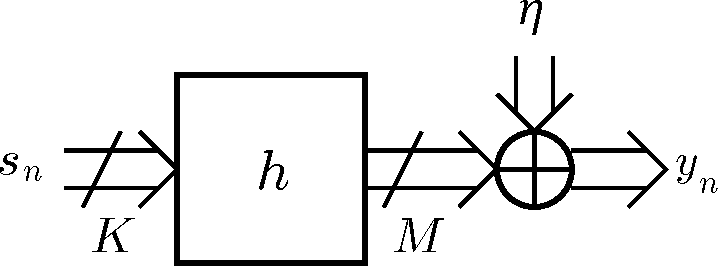
\includegraphics[width = 0.7\columnwidth]{channel}
	\end{center}
	System Model: $\vec y_n = \ma H \vec s_n + η_n$\\
	with $\ma H = (h_{m,k}) \in \C^{M \times K}$ \qquad ($m\in[1,M], k\in[1,K]$)\\
	\textbf{Linear Channel Model} $\vec y = \ma S \vec h + \vec n$ with \\$\vec h \sim \mathcal N (0, \ma C_{\vec h})$ and $\vec n \sim \mathcal N (0, \ma C_{\vec n})$\\
	\\
	Linear Estimator $\ma T$ estimates $\hat {\vec h} = \ma T \vec y \in \C^{MK}$\\
	$\ma T_{\ir MMSE} = \ma C_{\vec h \vec y} \ma C_{\vec y}^{-1} = \ma C_{\vec h} \ma S^{\ir H} (\ma S \ma C_{\vec h} \ma S^{\ir H} + \ma C_{\vec n})^{-1}$\\
	$\ma T_{\ir ML} = \ma T_{\ir Cor} = (\ma S^{\ir H} \ma C^{−1}_{\vec n} \ma S)^{-1} \ma S^{\ir H} \ma C_{\vec n}^{-1}$\\
	$\ma T_{\ir MF} ∝ \ma C_{\vec h} \ma S^{\ir H} \ma C_{\vec n}^{-1}$\\
	For Assumption $\ma S^{\ir H} \ma S = N σ_s^2 \ma 1_{K \times M}$ and $\ma C_{\vec n} = σ_η^2 \ma 1_{N\times M}$\\
	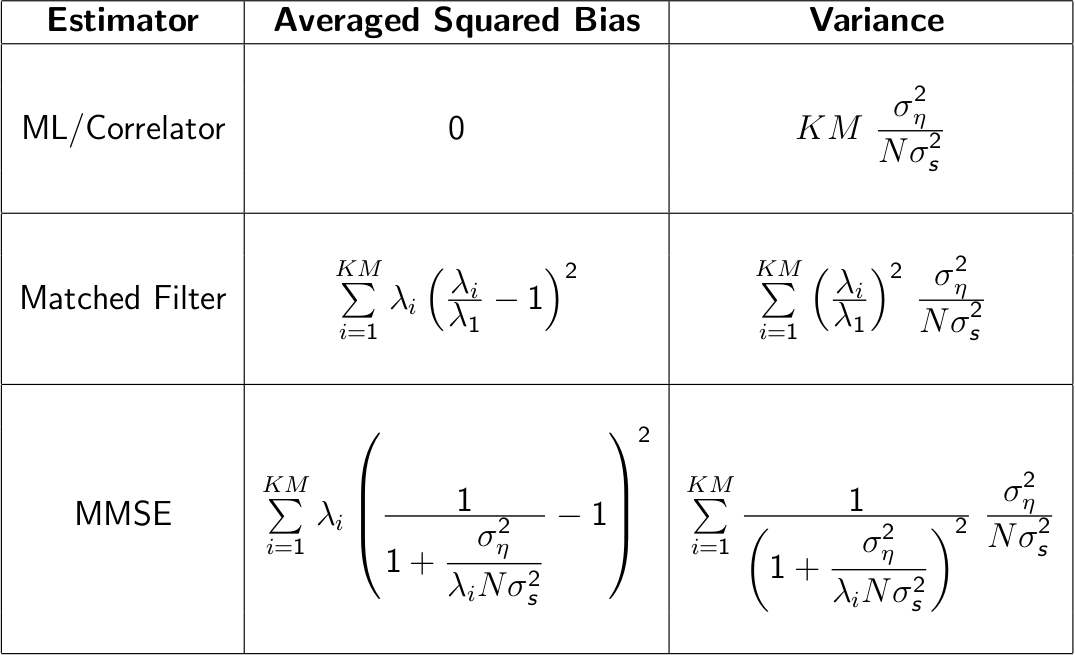
\includegraphics[width = \columnwidth]{comparison}
\end{sectionbox}




\begin{sectionbox}
	\subsection{Estimators}
	Upper Bound: Uniform in $[0;θ]: \hat{θ}_{\ir ML} = \frac{2}{N} \sum x_i$\\
	Probability $p$ for $\mathcal B(p,N)$: $\hat{p}_{\ir ML} = \frac{x}{N}$ \quad $\hat{p}_{\ir CM} = \frac{x+1}{N+2}$\\
	Mean $μ$ for $\mathcal N(μ,σ^2): \hat{μ}^2_{\ir ML} = \frac{1}{N} \sum\limits_{i=1}^N x_i$\\
	Variance $\sigma^2$ for $\mathcal N(μ,σ^2): \hat{σ}^2_{\ir ML} = \frac{1}{N} \sum\limits_{i=1}^N (x_i - μ)^2$

\end{sectionbox}

